\chapter{Introduction}\label{chapter:introduction}

Given growing demand, programming class sizes at major universities like MIT, Stanford, Berkeley, and University of Washington are reaching hundreds or thousands of students. However, one-on-one tutoring is considered a gold standard for the educational outcomes it regularly produces \cite{bloom}. The rapid, personalized feedback and attention that is possible within a one-on-one tutoring relationship or a small class becomes prohibitively difficult or expensive at larger scales. Systems and techniques that scale the benefits of low student-to-teacher ratios to arbitrarily many students is an on-going challenge in modern education.

Computers are a natural ally in this challenge. Even though computers do not yet have a human's ability to design curriculum, compose an entirely new question, or handle a novel answer, their attention, computation, and memory scales much better than humanity's. This thesis work supports a vision of teaching computer science education where humans--teachers and students--are front and center, discussing approaches, design choices, and trade-offs, augmented by computation behind the scenes.

The challenge of scaling up computer science education is usually framed as simply coping with the problems of large class sizes. This thesis, however, explores how the volume of students and their solutions can be exploited to enable new types of rapid personalized feedback, as well as recover aspects of a traditional small class.

Learners individually solving programming problems can collectively generate a wide variety of possible bugs and solutions. A single programming or digital hardware design exercise may yield thousands of student solutions that vary in many ways, some superficial and some fundamental. For teachers, this variation can, for example, be a source of pedagogically valuable examples and corner cases that slipped past an automatic grader. For students, the variation in a large class means that other students may have struggled along a similar solution path, hit the same bugs, and can offer hints based on that earned expertise. 

Understanding large-scale variation in student solutions requires identifying appropriate features of solutions, developing ways to automatically extract those features from each solution, designing user interfaces to communicate the results to teachers or students, and, when appropriate, collecting additional information from students through crowdsourcing techniques, i.e., learnersourcing \cite{kim2013learnersourcing}. This thesis includes the development of three systems that take advantage of the solution variation in large classes: OverCode for viewing thousands of Python solutions, Foobaz for delivering personalized feedback on variable names, self-reflection and comparison workflows for learnersourcing curcuit debugging and optimization hints. These systems and workflows, as well as an extension of OverCode adapted to grading, have been evaluated using data or live deployments in on-campus or edX courses with hundreds or thousands of students.


\section{The Status Quo}

Several years ago, I was hired as a teaching assistant in Computation Structures (6.004). This class is famous for its culminating semester-long project. To pass the class, every student must make an entire processor out of simulated logic gates. Much of my time was spent helping approximately 200 enrolled students debug their simulated circuits. This was fun, but it had several frustrating elements:

\begin{enumerate}
\item The simulated circuits were created by students using a language developed by the lecturing professor. It was difficult to read or skim.
\item Since student solutions were only evaluated based on input-output behavior, they could create many different innovative (or inefficient) designs. Established optimizations, like ripple carry adders, were discussed in class, but the diversity of good and bad designs found within our own crowd of students' solutions were never systematically examined. One student had the courage to publish his own innovative design on the course forum, and we teaching assistants spent much of the rest of the week helping everyone else understand and implement it. How many other students came up with an innovative idea but were afraid to share it, or did not even realize that it was new and different? Some students had no idea whether their solutions were common or unusual.
\item Students failed many of the same teacher-provided tests for the same reasons. These (test failure, problem) patterns would evolve in my mind as I helped more and more students. I was sometimes reduced to an inefficient middleman of debugging advice serving a long queue of customers, repeating myself and guessing problems: ``You failed test 286? Check your Z logic!'' The class forum did not seem to alleviate this problem, possibly because students did not encode their test failure problems in a consistent manner for easy searchability.
\end{enumerate}

The professor, who had created the course decades ago, had created multiple implementations of every major circuit design assignment over the years. He was the real resident expert. I shadowed him helping students like medical student might shadow a senior physician. And yet, in order to have the perspective he had without also spending decades teaching the same class, I wanted to augment my cognition with technology. 

\subsection{A Tale of Two Turing Machines}

I was wrapping up my late-night shift helping students in the computer lab, when a student asked for help with the Turing machine lab. His Turing machine could not detect whether a string of open and closed parentheses was properly balanced, i.e., had an appropriate closing parenthesis for every open parenthesis. He was running out of time. The semester was almost over, and if he was not successful within the next day or two, he would fail our course.

On that late night, I had a hard time helping this student turn his Turing machine into one that would pass all the autograder test cases. I could not tell whether his approach could work with a little debugging or was fatally flawed. I did not want to demoralize him by telling him to abandon his efforts so far and start over unless it was truly necessary. And what if he was on the path to a novel solution no one else had created before? While not a necessary condition for the correctness of his intended approach, finding a similar working solution in the pool of previous student submissions would serve as an existence proof and evidence that he should persevere. 

I had copies of hundreds of other students' correct Turing machines, but it was difficult to see by inspection whether any of these solutions were successful implementations of his intended approach. This was due to superficial differences between solutions: 
\begin{enumerate}
\item Students design their own symbol library and state names for the finite state machine portion of their Turing machine. 
\item Using their custom symbol and state names, students can list behavioral specifications in any arbitrary order. 
\item After translating these textual statements into a diagram, the diagrams can look very different from one correct solution to the next. 
\end{enumerate}
It is difficult to immediately see any differences in behavior or strategy based on these representations.

Eventually, through trial and error, he got his Turing machine to work on all the test cases, and passed the course. But I was deeply troubled by the experience. I felt like the information was there, in our staff server, but my brain could not see through the superficial textual differences nor mentally execute all the student solutions I had access to in order to have the perspective that would help me help students.

After the semester ended, I looked into this further. I ran all the correct two-state Turing machines collected during the semester on the same test tape containing a string of open and closed parentheses. The movement of the tape-reading head across this input was logged in coordinates relative to the common starting point at the left end of the test tape (see Figure \ref{tapeLocations}). I had watched so many students' Turning machines execute before that I knew there were be some patterns, I just did not know exactly what or how many there would be.

Most machines exhibited one of two common movement patterns. Roughly 50\% of students used Strategy A: pairing inner sets of open and closed parentheses (Figure \ref{tapeMoveA}). Another 40\% used Strategy B: pairing the first open with the first closed parenthesis, the second open with the second closed parenthesis, etc. (Figure \ref{tapeMoveB}). The bold trajectories in these figures represent particularly clean representative examples.

\begin{figure*}[p]

\begin{subfigure}[b]{1.0\textwidth}
\centering
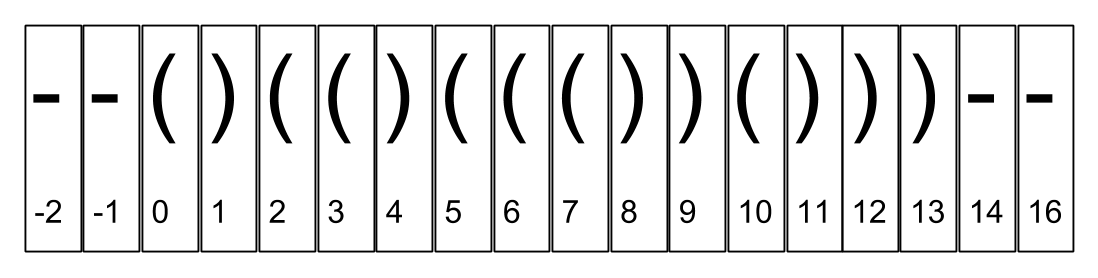
\includegraphics[width=140mm]{Body/figures/ICERtapeLocations.png}
\caption{Tape on which all 148 two-state Turing machines were tested, and the numbering system by which locations along the test tape are identified.}
\label{tapeLocations}
\end{subfigure}

\begin{subfigure}[b]{1.0\textwidth}
\centering
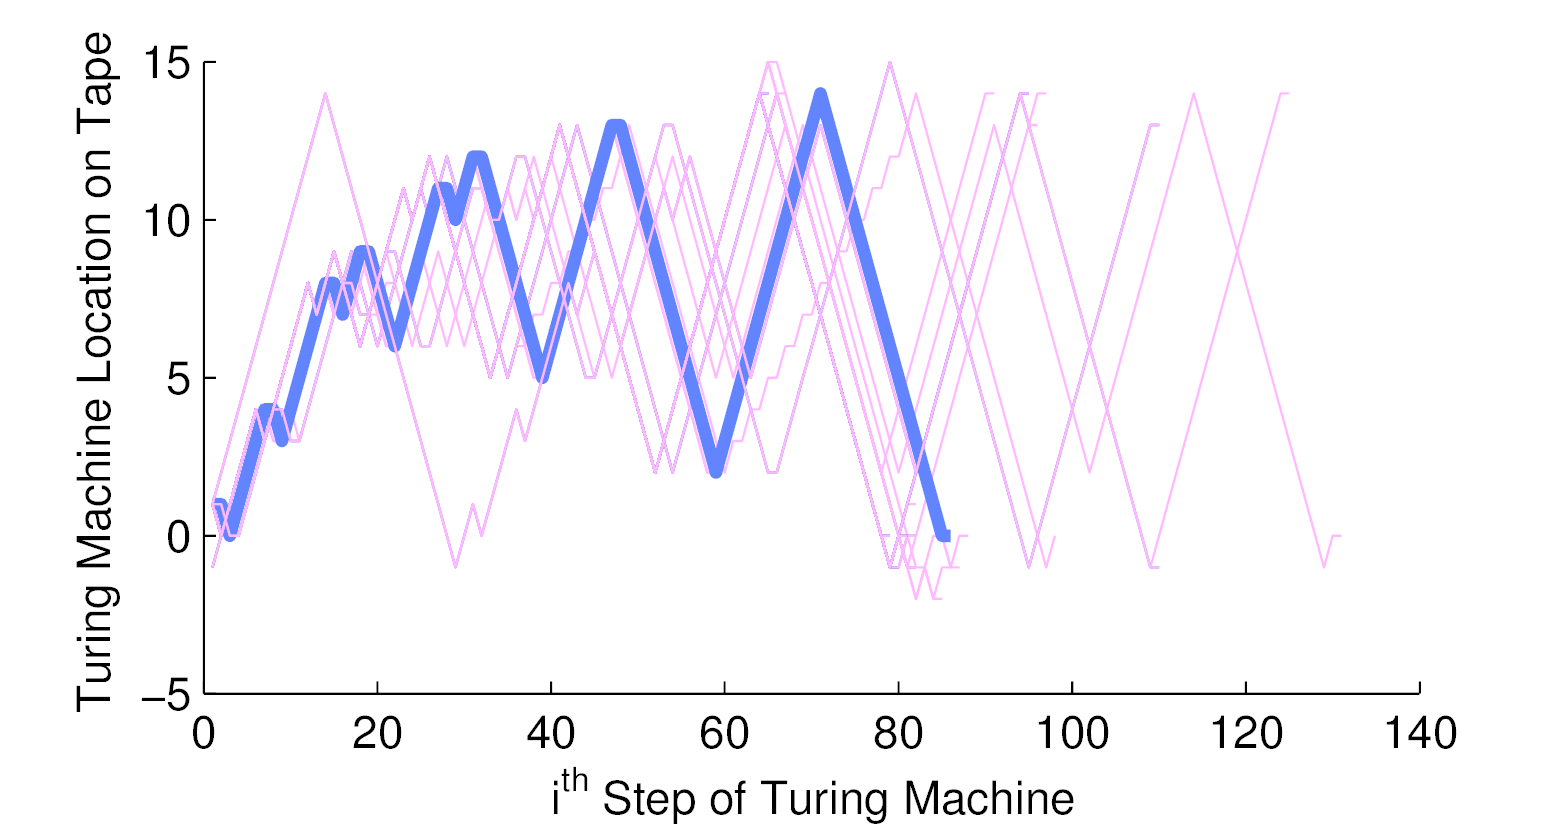
\includegraphics[width=0.85\textwidth]{Body/figures/tmvisualization_InnerParensMatched_allkidsAnno2}
\caption{Strategy A Turing machines: those which paired inner sets of open and closed parentheses, as is standard in mathematical notation. (73 out of 148 Turing machines)}
\label{tapeMoveA}
\end{subfigure}

\begin{subfigure}[b]{1.0\textwidth}
\centering
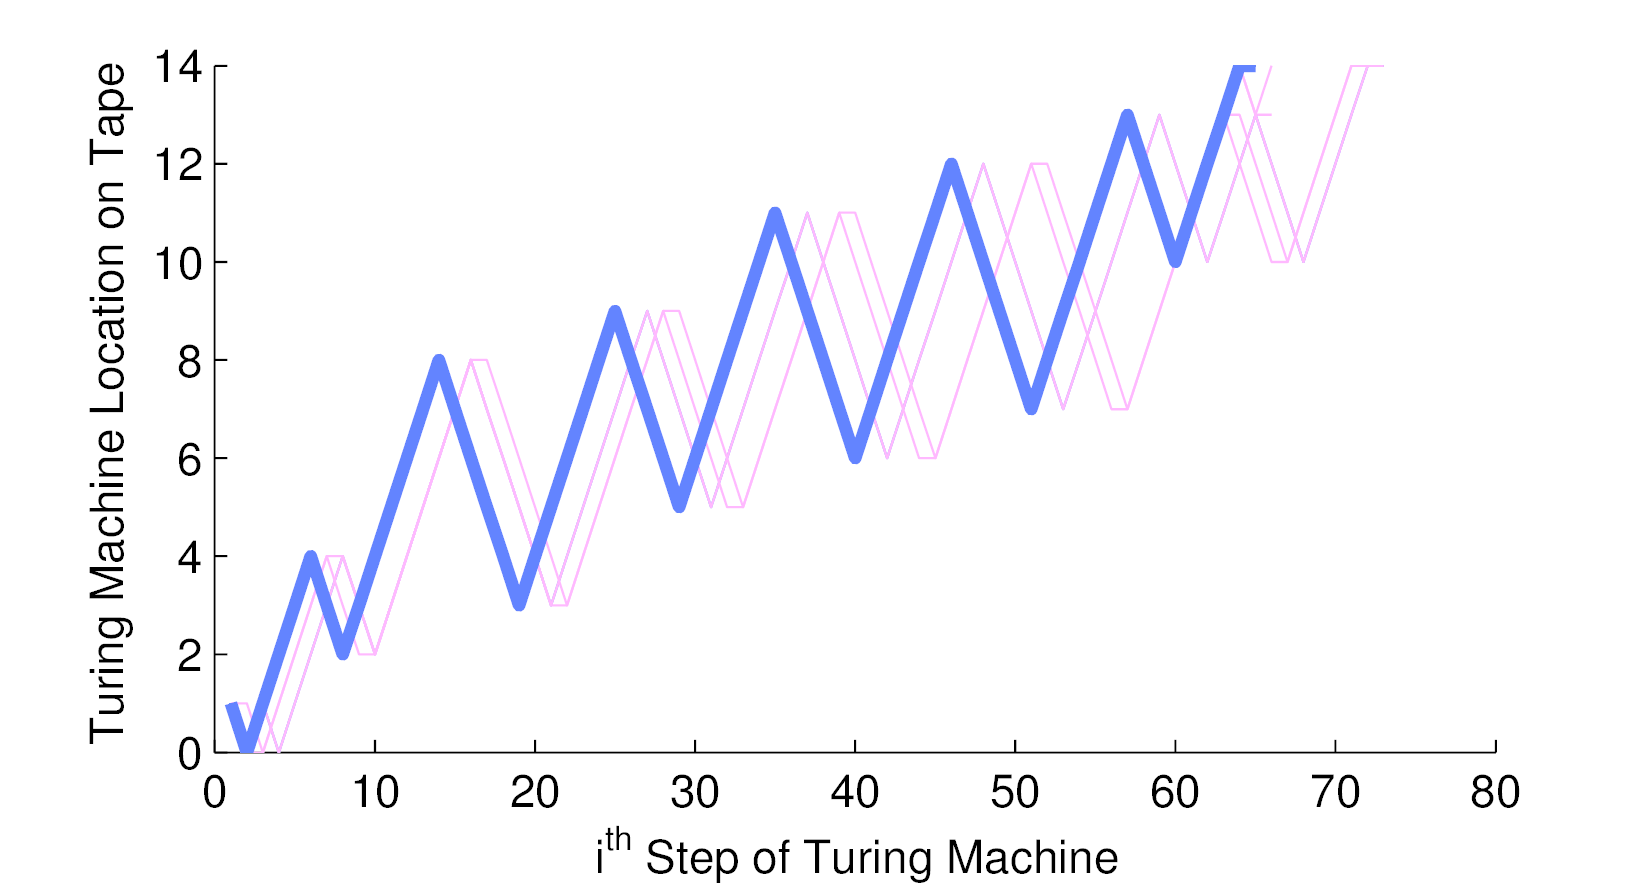
\includegraphics[width=0.85\textwidth]{Body/figures/tmvisualization_NtoNParensMatched_allkidsAnno2}
\caption{Strategy B Turing machines: those which paired the first open with the first closed parenthesis, the second open with the second closed parenthesis, etc. (58 out of 148 Turing machines)}
\label{tapeMoveB}
\end{subfigure}

\caption{The two most common strategies for a two-state Turing machine to determine if a string of parentheses is balanced. Figures \ref{tapeMoveA} and \ref{tapeMoveB} show tape head position over time on the tape illustrated in Fig. \ref{tapeLocations}. The bold trajectories represent particularly clean examples.}
\label{turingFig}
\end{figure*}

The remaining approximately 10\% solutions (not shown) include less common strategies, including at least two that are actually incorrect, i.e., cannot handle arbitrarily deep nesting of parentheses, but are marked as correct because they pass all the test cases in the teacher-designed suite. Many teaching staff members:
\begin{enumerate}
\item were aware of the Turing machine solution they each had found on their own time.
\item not aware that there were two mutually exclusive common solutions. At least one staff member admitted steering students away from solutions they did not recognize, but in retrospect may have indeed been valid solutions.
\item not aware that the test suite was insufficient to determine correctness.
\end{enumerate}

I was able to brief fellow staff members on the space of solutions, both good and bad, in preparation for subsequent semesters and suggested additions to the test tape suite to catch more submissions that were previously erroneously marked as correct.

\section{OverCode}

Understanding solution variation is important for providing appropriate feedback to students at scale. In one-on-one scenarios, understanding the space of potential solutions can help teachers counsel students struggling to implement their own solutions. The wide variation among these solutions can be a source of pedagogically valuable examples, and can be used to refine the autograder for the exercise by exposing corner cases. 

I acquired a dataset of thousands of correct student-written Python solutions to the same programming problem, freshly collected from MIT's introductory Python programming course on edX. Analogous to tracking Turing machine movement, my colleague Rishabh Singh and I realized that we could identify meaningful patterns in Python solutions by tracking the values of variables during execution on test cases. With the help of Philip Guo, who contributed variable value-logging code from his Online Python Tutor~\cite{pgbovineOPT} and Jeremy Scott, who built the user interface, we created and tested OverCode, a system for visualizing and exploring thousands of programming solutions.

OverCode uses both static and dynamic analysis to cluster similar correct solutions, and lets teachers further filter and cluster solutions based on different criteria. OverCode rewrites solutions to make them understandable as a collection. To do this, OverCode runs all the solutions to the same programming problem on the same test case(s) and extracts the sequence of values every variable in every solution takes on during execution. Variables that take on the same sequence of values across multiple correct solutions are assumed to be the same {\it common variable}. The most {\it common name} given to each {\it common variable} across all solutions is then used to rename all instances of that common variable in all solutions. At the same time, students' individual comments are removed and formatting is standardized. The resulting set of solutions are rendered in such a way that variable names are semantically meaningful and shared across solutions, as a common vocabulary. All solutions whose {\it set} of lines are the same after this normalization process are clustered together, and one of those normalized sets of lines will represent the entire cluster as the {\it platonic} solution. %A platonic solution represents the entire cluster.

We evaluated OverCode against a non-clustering baseline in a within-subjects study with 24 teaching assistants, and found that the OverCode interface allows teachers to more quickly develop a high-level view of student understanding and misconceptions, and to provide feedback that is relevant to more student solutions.

OverCode addressed the first two of my three frustrations as a teaching assistant:
\begin{enumerate}
\item It normalizes student code so that I can skim their answers as a group or as individuals without first adjusting to each of their variable naming, statement ordering, and style choices.
\item The diversity and distribution of good and bad designs generated by our students is made explicit and explorable. For example, OverCode shows common solutions, which are often reasonable since many students independently arrived at them, and as the user scrolls to less common solutions, solutions can become more convoluted, include unnecessary code, use reasonable alternative Python language keywords and constructs, or solve the problem using teacher-forbidden strategies, e.g., recursively rather than interatively.
\end{enumerate}

\begin{figure}
\centering
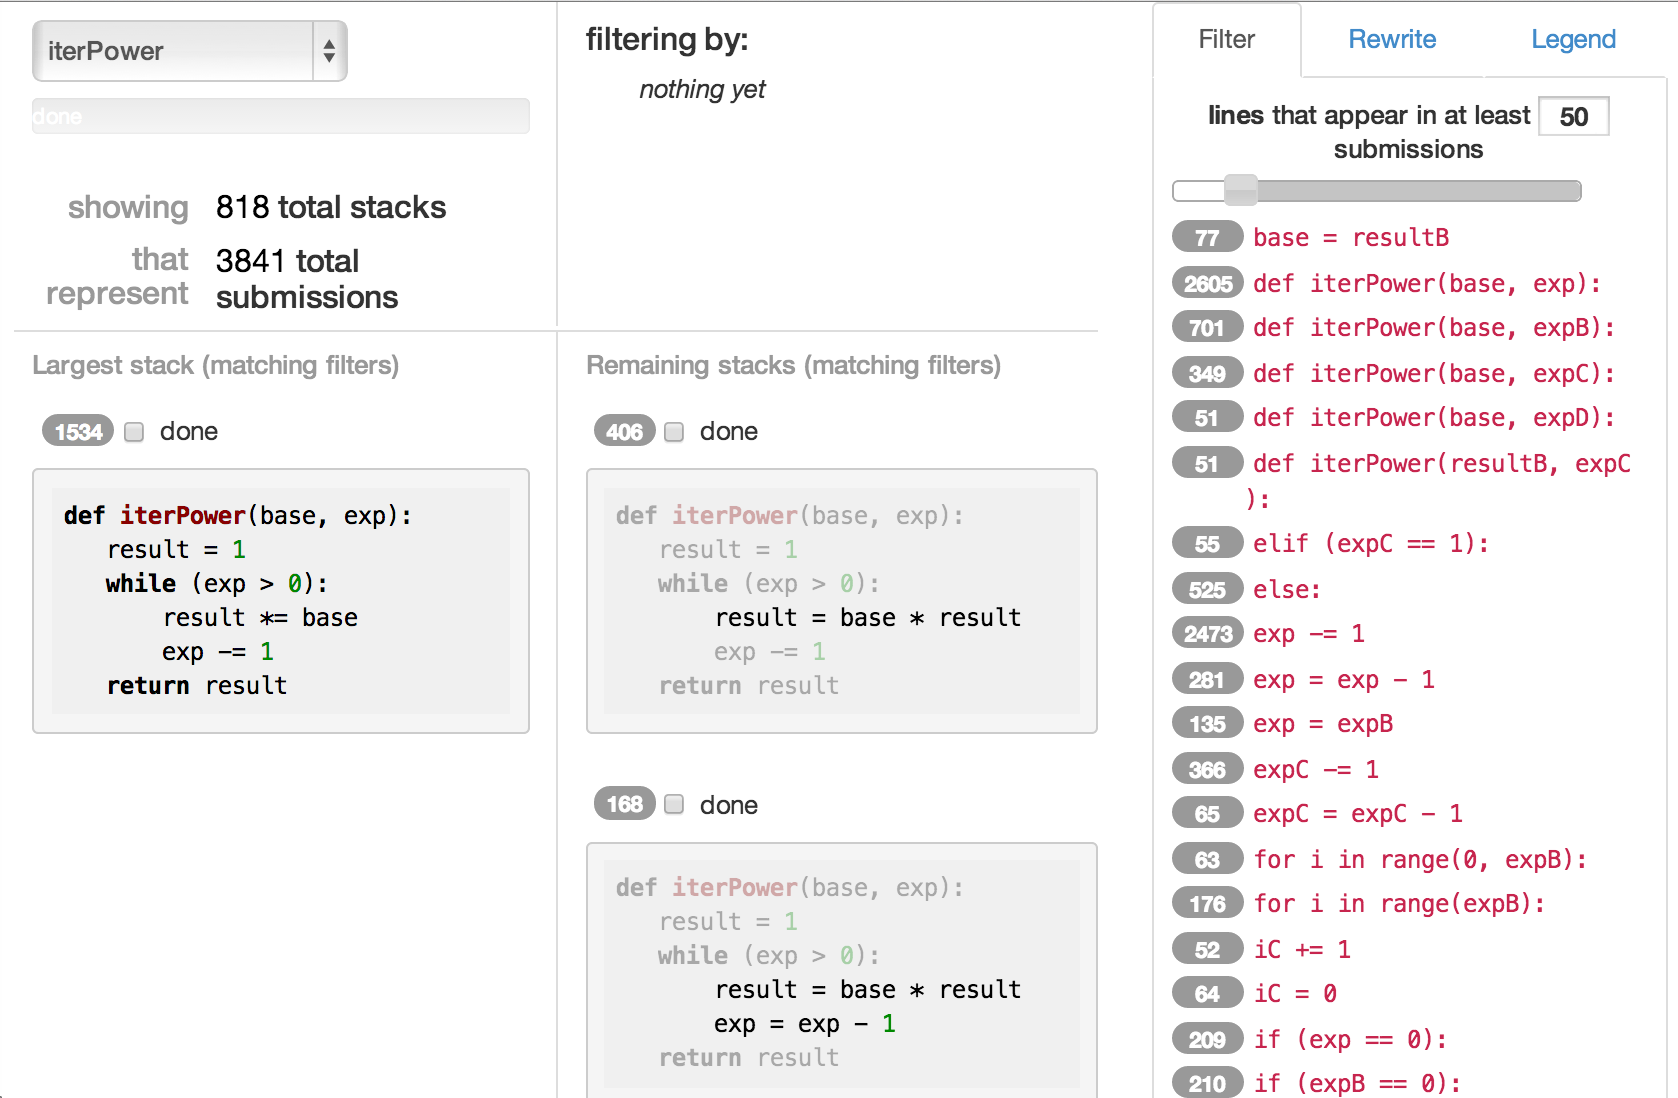
\includegraphics[width=1.0\linewidth]{Body/figures/interfaceScreenShot.png}
\caption{The OverCode user interface. The top left panel shows the number of clusters, called {\it stacks}, and the total number of solutions visualized. The next panel down in the first column shows the largest stack, while the second column shows the remaining stacks. The third column shows the lines of code occurring in the normalized solutions of the stacks together with their frequencies.}
\label{fullinterface}
\end{figure}


\section{Foobaz}

I approached Ana Bell, the lecturer who served both MIT's residential and online introductory Python programming courses. She found the OverCode interface interesting and hoped to use it, then asked if OverCode could also show her more about student variable name choices. In a second meeting, her co-teacher, Professor John Guttag, explained that some introductory students mix themselves up by creating names that suggest something other than what the variable contains, e.g., swapping names for the index into an array with the name for the value in the array at that index. It could be an innocent mistake that lengthens debugging time or indicative of a flawed mental model, and it can throw a wrench into their program comprehension process. 

Some programmers undervalue variable names, but they are the most basic form of documentation that helps humans read programs. Donald Knuth compares a good programmer to an essayist who, ``with thesaurus in hand, chooses the names of variables carefully and explains what each variable means'' \cite{literateprogramming}. Without modifying execution, names can express to the human reader the type and purpose of an object, as well as suggest what the kinds of operators used to manipulate it \cite{operands}. Various naming conventions, like Hungarian notation, have evolved to help developers use their freedom wisely. The Google C++ Style Guide authors assert that their most important consistency rules govern naming, which are arbitrary but consistent in order to increase human readability. 

Programmers can develop their own heuristics for good variable names through the experiential learning process of building, debugging, and sharing increasingly large programs with others and their future selves. During informal interviews with programmers in my social network, one professor explained an elaborate set of guidelines that she personally developed and teaches to her students, e.g., all method names must be verbs \cite{doshiconversation}.

In practice, very little time is spent on variable naming in introductory classes. One student-taught month-long introductory Python course offered at MIT spends one lecture on it, and does not systematically assess student naming choices afterwards. With new tools, giving feedback on variable names could become time-efficient and scalable enough to become common place. 

Building on top of OverCode and the support of my co-authors Jeremy Scott and Lyla Fischer, I designed and implemented Foobaz, a system that enables time-efficient, scalable, personalized variable name feedback within the context of existing assigned programming problems. OverCode systematically hid the variation in variable names. Foobaz reveals that variation, in context. %In addition, the new system can provide mechanisms for teachers to comment on the variation with the interface and deliver that commentary to students in a personalized way. 

Like OverCode, Foobaz distinguishes variables by their behavior, recognizing {\it common variables}. For each common variable, Foobaz allows teachers to comment not only on poor names, but also on names that mislead the reader about the variable's role. As shown in Figure \ref{fig:foobaz_teacherview}, the teacher view is a variable name browser where names are shown along with all the context necessary to judge their quality. Teachers only need to annotate a small number of variable names with qualitative judgements in order to generate personalized formative assessments about variable naming for the majority of their students.

In our first user study, the Foobaz system helped each of ten teachers give personalized variable name feedback on thousands of student solutions from the MIT introductory Python programming course on edX. In the second study, students composed solutions to the same programming assignments and immediately received personalized quizzes composed by the teachers in the previous user study, like the one shown in Figure~\ref{fig:foobaz_studentview}.

Traditional feedback methods, such as hand-grading student code for substance and style, are labor intensive and do not scale. Foobaz addresses feedback at scale for a particular and important aspect of code quality. Foobaz also addressed the second of my three frustrations as a teaching assistant: making the diversity and distribution of good and bad choices explicit. %But what about my last frustration as a teaching assistant, about helping students even get to a correct solution?

\begin{figure*}[p]

\begin{subfigure}[b]{1.0\textwidth}
\centering
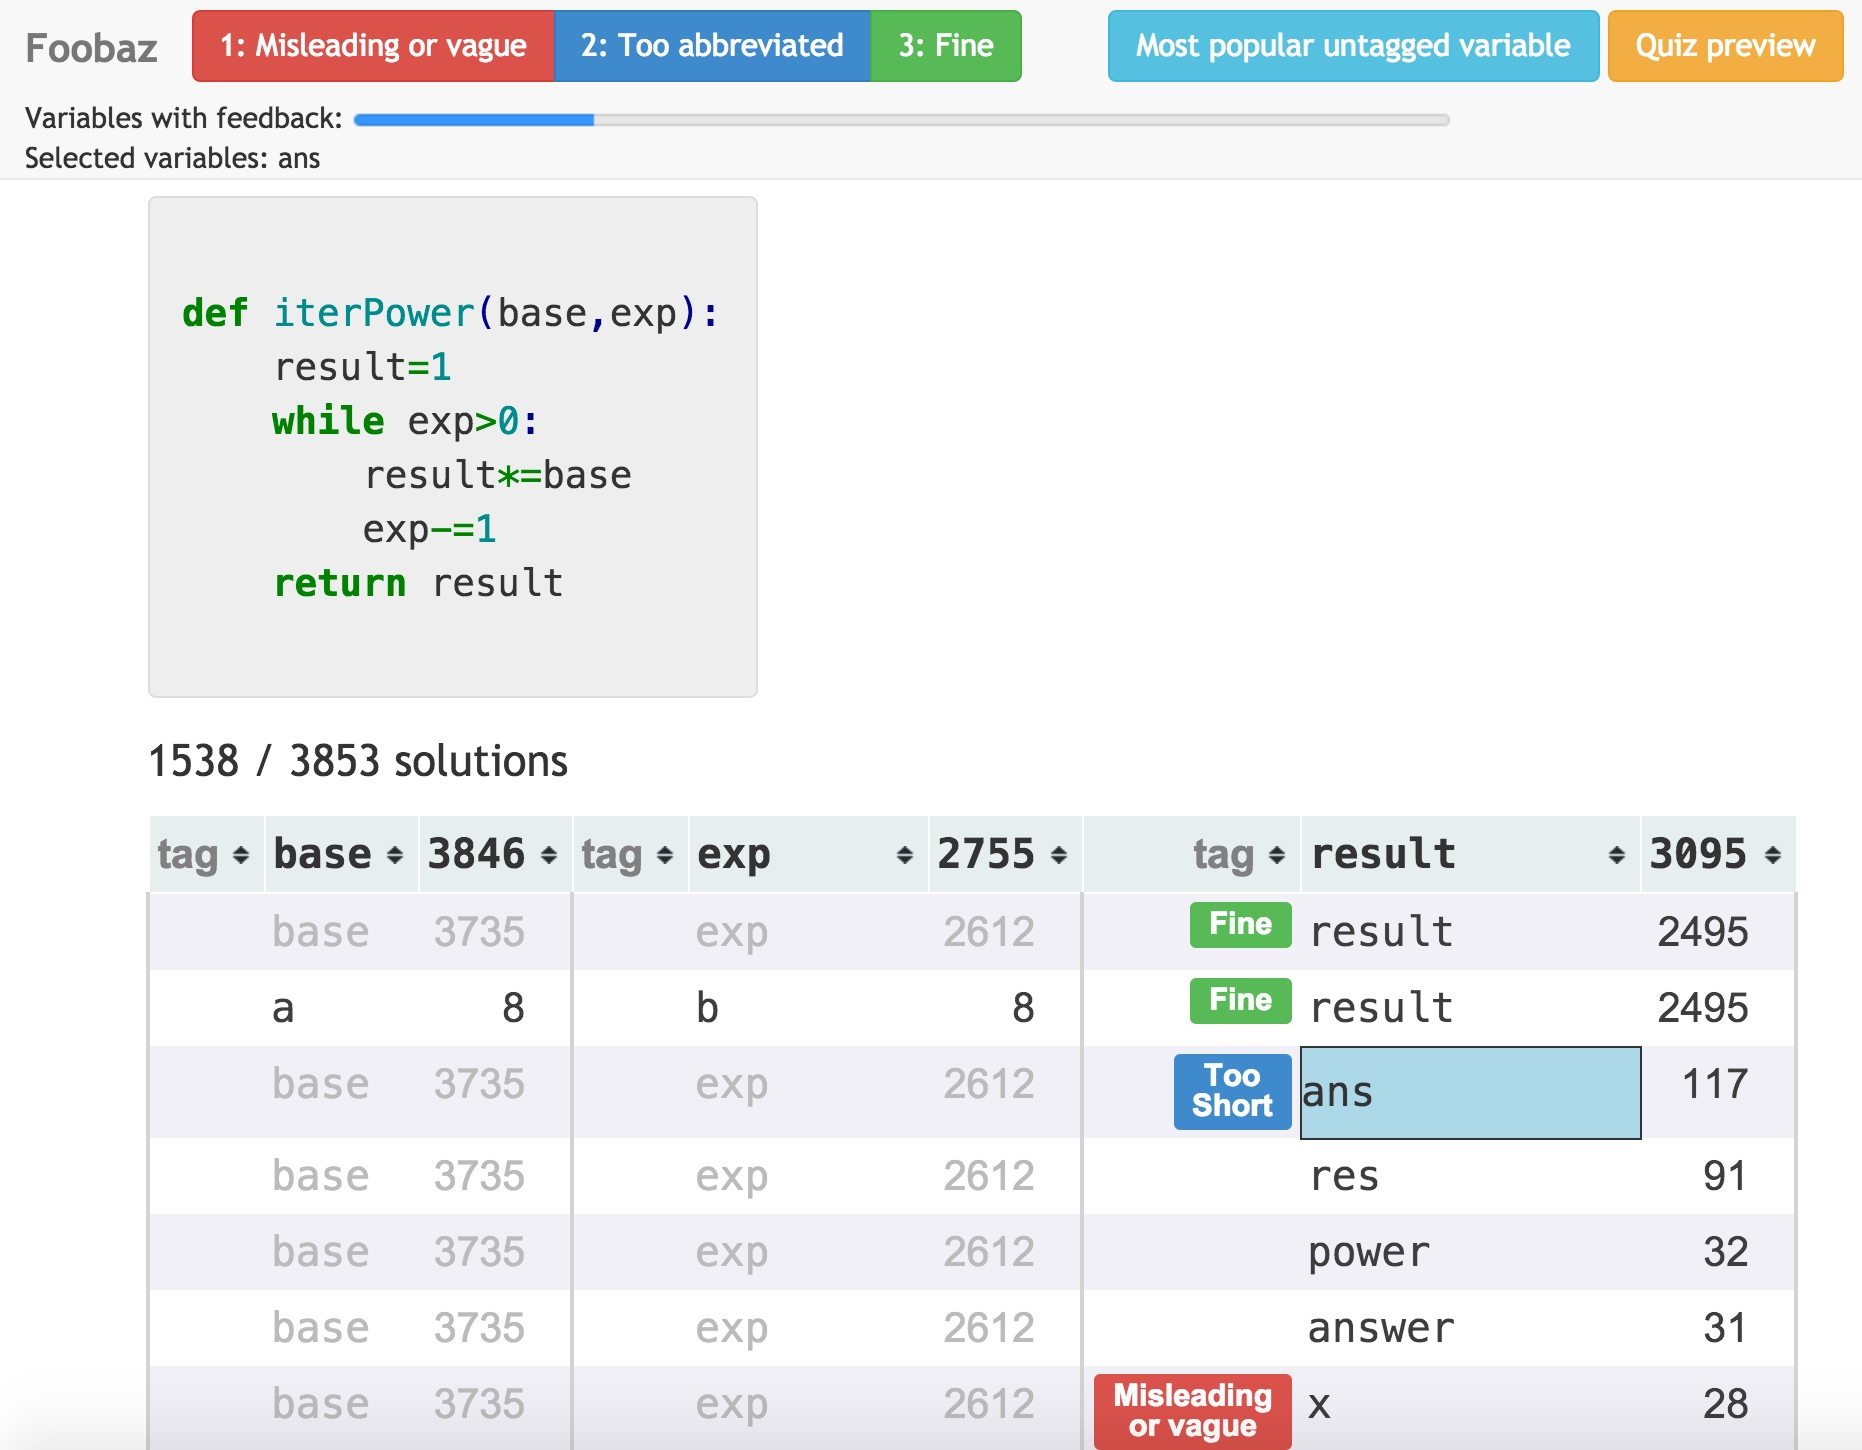
\includegraphics[width=0.75\linewidth]{Body/figures/foobaz/FoobazInitialView4.jpg}
\caption{The Foobaz teacher interface. The teacher is presented with a scrollable list of normalized solutions, each followed by a table of student-chosen variable names. Some names shown here have been labeled by the teacher as ``misleading or vague,'' ``too short,'' or ``fine.''}
\label{fig:foobaz_teacherview}
\end{subfigure}

\begin{subfigure}[b]{1.0\textwidth}
\centering
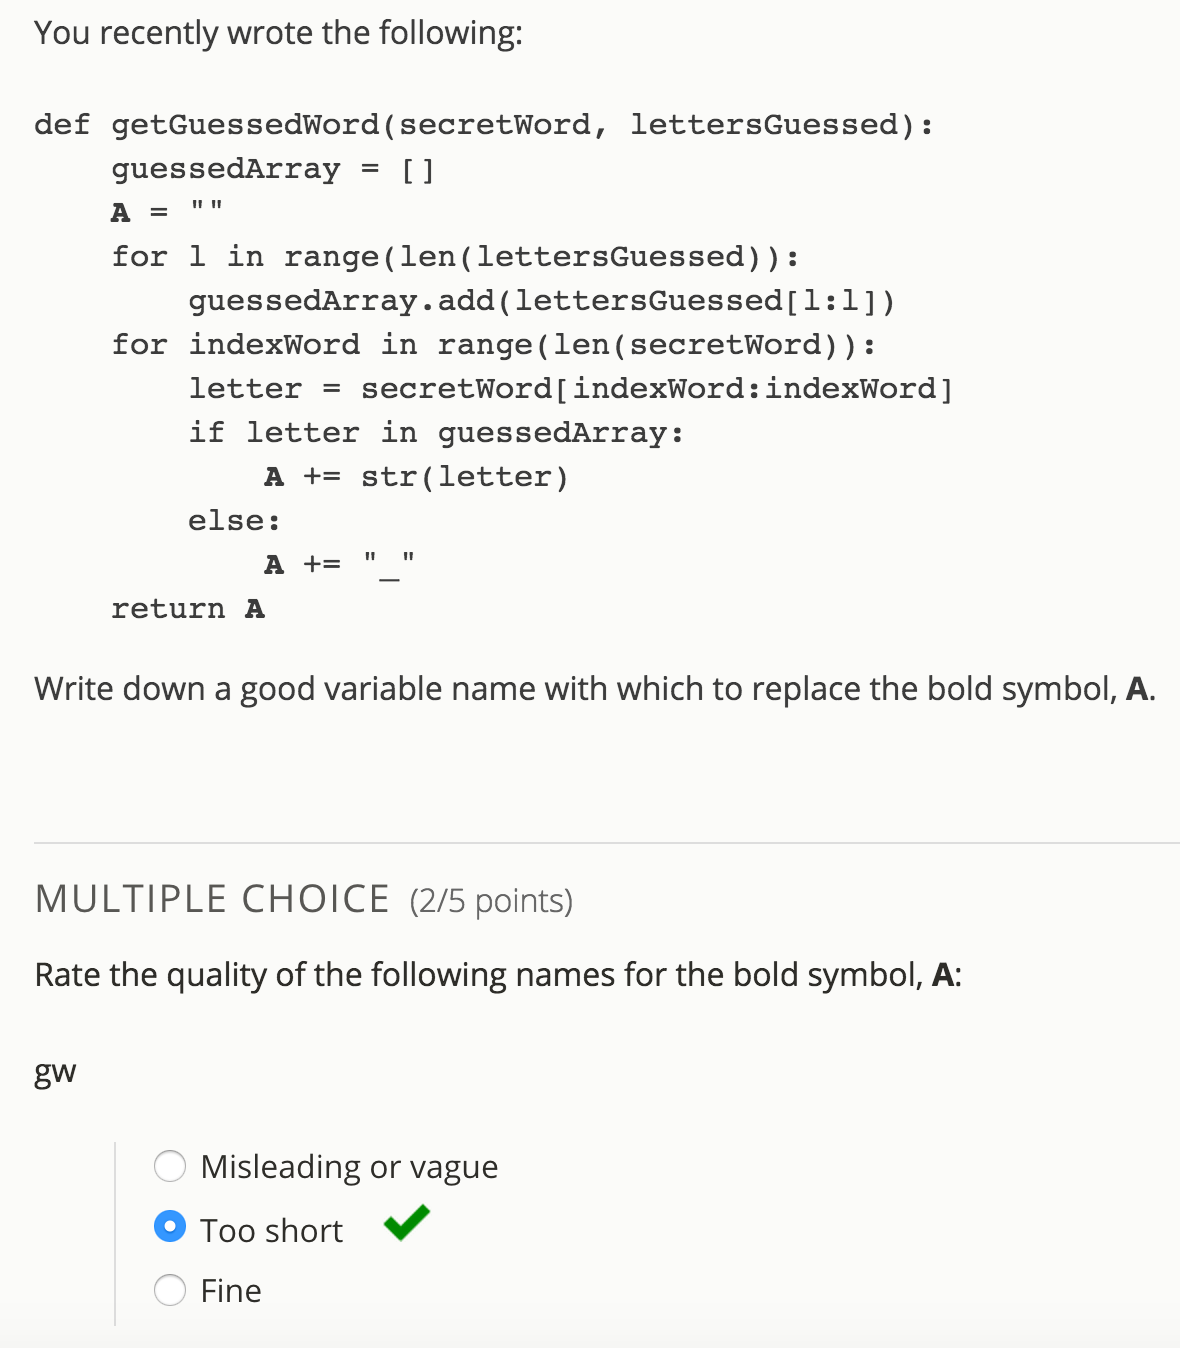
\includegraphics[width=0.4\linewidth]{Body/figures/foobaz/feedbackQuizExample.png}
\caption{A personalized quiz as seen by the student, delivered by edX infrastructure. Students are shown their own code, with a variable name replaced by an arbitrary symbol, followed by variable names for the student to consider and label using the same labels that were available to the teacher. After the student has submitted their own judgments, the teacher’s labels are revealed, along with their explanatory comments.}
\label{fig:foobaz_studentview}
\end{subfigure}

\caption{Snapshots of the Foobaz teacher interface and student variable name quiz}
\end{figure*}
\todo{replace quiz screenshot with system screenshot}


\section{Self-Reflection and Comparison Workflows}

%It is not unreasonable to focus on correct solution in an environment when many students in introductory programming classes can repeatedly check their code against teacher-designed test suites until it passes. However, based on personal experience, a large fraction of teachers' time, especially in residential environments, is spent helping students get to a correct solution. Personalized support for students is a gold standard in education, but it scales poorly with the number of students. %Prior work on \textit{learnersourcing} presented an approach for learners to engage in human computation tasks while trying to learn a new skill.

The final section of this thesis is a response to another personal experience in the lab as a teaching assistant, paraphrased here:
\begin{displayquote}
    Student A: ``I cannot figure out why I'm having this bug.''

    Teacher (me): ``Oh, I have not seen this behavior before. Strange...''

    {\it We sit together, brainstorming, trying things, debugging, stuck...}

    Student B walks in, overhears us: ``Oh, I just had that buggy behavior. Have you considered...?''
\end{displayquote}
They had separately created the same bug, one after the other. Student B helped Student A debug it. By random chance or because I am not a novice, I had not generated that problem in my own code before. I could model good debugging skills, but Student B could be just as, if not more, helpful to Student A. Student B had earned expertise through experience that I had not. As demonstrated in the user studies that follow, students can and do often restrain themselves from giving away the answer when asked to generate a hint after struggling to correct a bug or finish an implementation. 

Shortly after my experience of coincidental peer teaching, I stopped thinking of myself as a resident expert and started thinking about how to help students more directly share their earned expertise with other students, in a way that would be beneficial for both the giver and the receiver. After helping each student fix a bug and observe a test case go from failed to passed, I asked the student to compose a hint for other students like them who are still failing the same test. I then asked them to enter that hint, indexed by the id of the test case it might resolve, in a web application I wrote, where it would be accessible to all students in the course. Other teaching assistants started pointing students to the web application before helping them, to decrease repeating themselves. I also released it to edX students taking the same course online. 

When I saw two students with complementary optimizations of an adder circuit, I made them teach each other their respective optimizations before I gave them their required lab check off. Then I pushed on toward automating this peer-to-peer help on optimalizing circuits. I used the number of transistors in the circuit (circuit size) as an approximate metric of optimality, examined the space of solutions as a function of circuit size, and picked out several key points on that landscape. 

During a later semester, when each student enrolled in Computation Structures submitted a correct adder circuit, they were automatically shown a slightly more optimal student solution and a slightly less optimal student solution. They then had to write hints about (1) how to turn a solution like theirs into the more optimal solution, forcing them to engage with and hopefully learn from a more optimal solution and (2) how to turn a solution like the less optimal solution into a more optimal solution like theirs, using their earned implementation expertise in the process. 

My co-authors and I hand-analyzed hundreds of optimization hints collected through these targeted prompts and categorized them into the types of hints an expert might write when going through the expensive process of building an intelligent tutoring system for this domain. In a small lab study, we found that students enrolled in later semesters of the same course could improve their own solutions based on these hints written for solutions like theirs by other students who had the experience to write them. 

In general, students in engineering courses can create many different solutions to the same problem, and the space of possible bugs accumulated over all paths to each solution can be very large. Teachers can model good debugging strategies and give feedback on a solutions they have not themselves already created, but students, through their own experience struggling with a particular problem, can become experts on the particular optimizations they implement or bugs they resolve. %The students can generate hints for fellow students based on their new expertise. 

In summary, I designed two workflows to harvest and organize students' collective knowledge and advice for helping fellow novices through design problems in engineering (see Figure \ref{fig:workflow}). Unlike general learnersourcing, this targeted form of learnersourcing allows or prompts specific students to help current or future students on challenges they have already conquered. In the process of participating in the workflows, students engage in self-reflection, self-explanation, and comparison with alternatives, hopefully within their zone of proximal development. The literature described in the chapter on Related Work suggests that these activities promote learning. Both workflows were evaluated in an undergraduate digital circuit design class with hundreds of students. Within these targeted learnersourcing workflows, students can create helpful hints for their peers that augment or even replace teachers' personalized assistance, especially when that assistance is not available. 

By taking better advantage of the knowledge distributed across many students, these workflows addressed the third and final of my three frustrations as a teaching assistant. Using these workflows, I hope future teaching assistants feel less like inefficient middlemen and more like the efficient debugging and optimization consultants they can be, augmented by explicit knowledge of the space of common and uncommon bugs and optimizations.%, by taking advantage of the knowledge distributed across many students.

%To take advantage of students' earned expertise, 
%The self-reflection workflow attempts to streamline the informal peer-debugging moment I saw in the lab. In the comparison workflow, this is generalized to peer-optimization of working solutions; students write hints about solutions slightly better and slightly worse than theirs. 

%Both workflows were evaluated in an undergraduate digital circuit design class with hundreds of students. We show that, within these targeted learnersourcing workflows, students can create helpful hints for their peers that augment or even replace teachers' personalized assistance, especially when that assistance is not available.

\begin{figure}
\centering
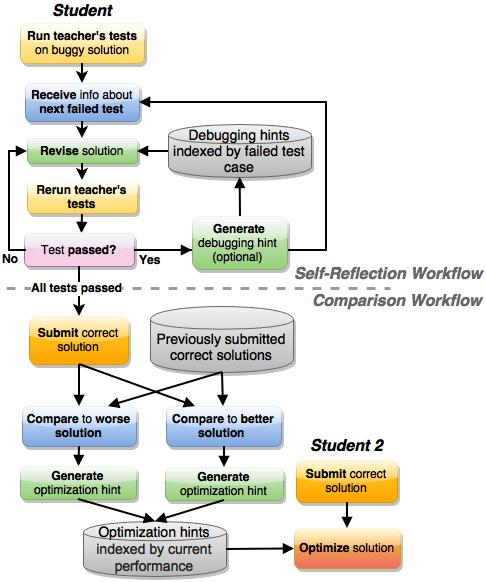
\includegraphics[width=1.0\linewidth]{Body/figures/classoverflow/CombinedWorkflow_CameraReady_FIXED_2.jpg}
\caption{In the \textit{self-reflection} workflow, students generate hints by reflecting on an obstacle they themselves have recently overcome. In the \textit{comparison} workflow, students compare their own solutions to those of other students, generating a hint as a byproduct of explaining how one might get from one solution to the other.}
\label{fig:workflow}
\end{figure}


\section{Additional Clustering and Visualization}

To further explore the power of clustering and visualizing solutions, several extensions of the OverCode methods were explored and one variant, GroverCode for grading, has been fully implemented. Adapting to the needs of a team of graders grading a smaller number of more complex solutions, many of which were incorrect, required significant changes to the pipeline and interface. The resulting system was deployed to the staff for use during two grading sessions. The results of this field deployment are also promising. The staff welcomes its continued use in future semesters. More preliminary explorations of statistical methods, such as Bayesian inference, for clustering solutions are explored (see Chapter ~\ref{chapter:grovercode}.



\section{Thesis Statement and Contributions}

The systems described in this thesis show various mechanisms for leveraging students in massive programming courses. Learners produce many variations of solutions to a problem, running into common and uncommon bugs along the way. Learners can be pure producers whose solutions are analyzed and displayed to teachers to augment their cognition and help them generate feedback. Alternatively, students can be prompted to generate analysis of their own and others' solutions, for the benefit of both themselves and current and future students. %, and sends it to selected fellow learners as feedback. %We would like to demo these systems together, as a suite of learnersourcing systems that allow teachers to turn the challenges of teaching at scale into an opportunity for discussion, self-reflection, peer-teaching, and more learning from examples.

My thesis statement is: 
\begin{displayquote}
Clustering and visualizing solution variation collected from programming courses can help teachers gain insights into student design choices, detect autograder failures, award partial credit, use targeted learnersourcing to collect hints for other students, and give personalized style feedback at scale.
\end{displayquote}

The main contributions of this thesis are:
\begin{itemize}
\item A novel visualization that shows similarity and variation among thousands of Python solutions, with normalized code shown for each variant. 
\item An algorithm that uses the behavior of variables to help cluster Python solutions and generate the normalized code for each cluster of solutions.
\item Two user studies that show this visualization is useful for giving teachers a birds-eye view of thousands of students' Python solutions.
\item A grading interface that shows similarity and variation among Python solutions, with faceted browsing so that users can filter solutions by error signature, i.e., the test cases they pass and fail. 
\item Two field deployments of the grading interface within introductory Python programming exam grading sessions.
\item A technique for displaying clusters of Python solutions with only an aspect, i.e., variable names and roles, of each cluster exposed, revealing the details that are relevant to the task. %In this application, the relevant features are variable names and roles.
\item A workflow for generating personalized active learning exercises, emulating how a teacher might socratically discuss good and bad choices with a student while they review the student's solution together. 
\item An implementation of the above technique and method for variable naming. % within datasets from both MOOCs and large residential classes on introductory Python programming.
\item Two lab studies which evaluate both the teacher and student experience of the workflow applied to variable names.
\item A self-reflection learnersourcing workflow in which students generate hints for each other by reflecting on an obstacle they themselves have recently overcome while debugging their solution to a Python or digital design exercise.
\item A comparison learnersourcing workflow in which students generate design hints for each other by comparing their own solutions to alternative designs submitted by other students.
\item A deployment of the self-reflection workflow in a 200-student class and a lab study of the comparison workflow with 9 participants.
\end{itemize}

\section{Thesis Overview}

Chapter \ref{chapter:relatedwork} summarizes prior and contemporary relevant research on systems that support programming education. It also briefly explains theories from the learning sciences and psychology literature that influenced or support the pedagogical value of the design choices made within this thesis.

The four chapters that follow describe, in detail, the four systems developed, as well as their evaluation on archived data or in the field.

\begin{itemize}
\item OverCode (Chapter \ref{chapter:overcode}) visualizes thousands of programming solutions using static and dynamic analysis to cluster similar solutions. It lets teachers quickly develop a high-level view of student understanding and misconceptions and provide feedback that is relevant to many student solutions. 

\item Foobaz (Chapter \ref{chapter:foobaz}) clusters variables in student programs by their names and behavior so that teachers can give feedback on variable naming. Rather than requiring the teacher to comment on thousands of students individually, Foobaz generates personalized quizzes that help students evaluate their own names by comparing them with good and bad names from other students. 

\item Chapter \ref{chapter:classoverflow} describes two workflows that collect and organize solution hints indexed by (1) the autograder test that failed or (2) a performance characteristic like size or speed. It helps students reflect on their debugging or optimization process, generates hints that can help other students with the same problem, and could potentially bootstrap an intelligent tutor tailored to the problem.

\item OverCode Extensions (Chapter \ref{chapter:grovercode}) describes (1) GroverCode, an extension to OverCode optimized for processing and displaying incorrect as well as correct student submissions and (2) clustering and mixture modeling algorithms applied to the OverCode pipeline output for additional insight into patterns within student solutions. 
\end{itemize}

Chapter \ref{chapter:discussion} discusses the design lessons that apply to the entire collection of systems in this thesis. Chapter \ref{chapter:conclusion} outlines avenues of future work this thesis work, in combination with the complementary work of others in this space, paves the way for.